\chapter{Aplicações da ORP 2} \label{apendice:orp2}

\section{Lista 1 - ORP2} \label{orp2l1}
\begin{itemize}
    \item[1.] \textbf{\cite{Halliday2009vol2}} Uma massa $M$ é dividida em duas partes, $m$ e $M-m$, que são em seguida separadas por certa distância. Qual é a razão $m/M$ que maximiza o módulo da força gravitacional entre as partes?

    \item[2.] \textbf{\cite{Halliday2009vol2}} Na figura abaixo, um quadrado com $20,0$ $cm$ de lado é formado por quatro esferas de massas $m_1=5,00$ $g$, $m_2 = 3,00$ $g$, $m_3 = 1,00$ $g$ e $m_4 = 5,00$ $g$. Na notação dos vetores unitários, qual é a força gravitacional exercida pelas esferas sobre a esfera central de massa $m_5 = 2,50$ $g$?
\begin{figure}[H]
\begin{center}
\caption*{Desenho Questão 2.}
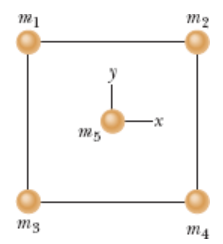
\includegraphics[width=0.3\textwidth]{fig/orp2l1q2.png}
\label{fig:ORP2q2}
\caption*{Fonte: \citeonline{Halliday2009vol2}}
\end{center}
\end{figure}

    \item[3.] \textbf{\cite{Halliday2009vol2}} A figura abaixo mostra duas cascas esféricas concêntricas homogêneas de massas $M_1$ e $M_2$. DEtermine o módulo da força gravitaconal a ue está sujeita uma partícula de massa $m$ situada a uma distância (a) $a$, (b) $b$ e (c) $c$ do centro comum das cascas.

\begin{figure}[H]
\begin{center}
\caption*{Desenho Questão 3.}
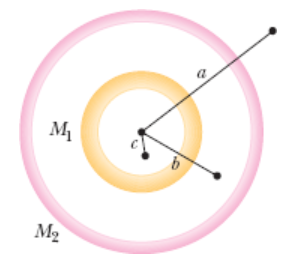
\includegraphics[width=0.3\textwidth]{fig/orp2l1q3.png}
\label{fig:ORP2q3}
\caption*{Fonte: \citeonline{Halliday2009vol2}}
\end{center}
\end{figure}

    \item[4.] \textbf{\cite{Halliday2009vol2}} Marte e a Terra tem diâmetros médios de $6,9 \times 10^3$ $km$ e $1,3 \times 10^4$ $km$, respectivamente. A massa de Marte é $0,11$ vezes a massa da Terra. Qual é a razão entre as massas específicas médias de Marte e da Terra? (b) Qual é o valor da aceleração gravitacional em Marte? (c) Qual é a velocidade de escape em Marte?

    \item[5.] \textbf{\cite{Halliday2009vol2}} Fobos, um satélite de Marte, se move em uma órbita aproximadamente circular com $9,4 \times 10^6$ $m$ de raio e um período de $7h39min$. Calcule a massa de Marte a partir dessas informações.

    \item[6.] \textbf{\cite{Halliday2009vol2}} A Figura abaixo mostra uma cavidade eférica no interior de uma esfera de chumbo de raio $R=4,00$ $cm$; a superfície da cavidade passa pelo centro dessa esfera e "toca" o lado direito da esfera. A massa da esfera antes de ser criada a cavidade era $M=2,95$ $kg$. Com que força gravitacional a esfera de chumbo com a cavidade atrai uma pequena esfera de massa $m=0,431$ $kg$ que está a uma distância $d=9,00$ $cm$ do centro da esfera de chumbo, na reta que passa pelo centro das duas esferas e pelo centro da cavidade?

\begin{figure}[H]
\begin{center}
\caption*{Desenho Questão 6.}
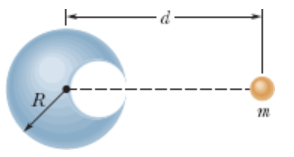
\includegraphics[width=0.3\textwidth]{fig/orp2l1q6.png}
\label{fig:ORP2q6}
\caption*{Fonte: \citeonline{Halliday2009vol2}}
\end{center}
\end{figure}

    \item[7.] \textbf{\cite{Halliday2009vol2}} Um planeta é modelado por um núcleo de raio $R$ e massa $M$ cercado por uma casca de raio interno $R$, raio externo $2R$ e massa $4M$. Se $M= 4,1 \times 10^{24}$ $kg$ e $R = 6,0 \times 10^6$ $m$, qual é a aceleração gravitacional de uma partícula em pontos situados a uma distância (a) $R$ e (b) $3R$ do centro do planeta?

    \item[8.] \textbf{\cite{Halliday2009vol2}} Zero, um planeta hipoético, tem massa de $5,0 \times 10^{23}$ $kg$, um raio de $3,0 \times 10^6$ $m$ e nenhuma atmosfera. Uma sonda espacial de $10$ $kg$ deve ser lançada verticalmente a partir da superfície. (a) Se a sonda for lançada com uma energia inicial de $5,0 \times 10^7$ $J$, qual será a energia cinética da sonda quando ela estiver a $4,0 \times 10^6$ $m$ do centro de Zero? (b) Com que energia cinética a sonda deverá ser lançada para atingir uma distância máxima de $8,0 \times 10^6$ $m$ em relação ao centro de Zero?

    \item[9.] \textbf{\cite{Halliday2009vol2}} Uma estrela de nêutrons típica tem massa igual à do So e raio de $10$ $km$. (a) Qual é a aceleração da gravidade na superfície da estrela? (b) COm que velocidade um objeto estaria se movendo se caísse a partir do repouso por uma distância de $1,0$ $m$ em direção à estrela? (Suponha que o movimento de rotação da estrela seja desprezível.)

    \item[10.] \textbf{\cite{Halliday2009vol2}} As massas e as coordenadas de três esferas são as seguintes: $20$ $kg$, $x = 0,50$ $m$, $y=1,0$ $m$; $40$ $kg$, $-1,0$ $m$, $y= -1,0$ $m$; $60$ $kg$, $x= 0$ $m$, $y= -0,5$ $m$. Qual é o módulo da força gravitacional que as três esferas exercem em uma esfera de $20$ $kg$ localizada na origem?

    \item[11.] \textbf{\cite{Halliday2009vol2}} Um objeto de massa $m$ é mantido inicialmente no lugar a uma distância $r=R_T$ do centro da Terra, em que $R_T$ é o raio da Terra. Seja $M_T$ a massa da Terra.  Uma força é aplicada ao objeto para deslocá-lo até uma distância $r=4R_T$, na qual é novamente mantido no lugar. Calcule, integrando o módulo da força, o trabalho realizado durante o deslocamento.

\end{itemize}
\newpage
\section{Lista 2 - ORP2} \label{ch:orp2l2}

\begin{itemize}
\item[1.] \textbf{\cite{Halliday2009vol2}} Uma janela de um escritório tem $3,4$ $m$ de largura por $2,1$ $m$ de altura. Como resultado da passagem de uma tempestade, a pressão do ar do lado de fora do edifício cai para $0,96 atm$, mas no interior do edifício permanece em $1,0$ $atm$. Qual é o módulo da força que empurra a janela por causa da diferença de pressão?


\item[2.] \textbf{\cite{Halliday2009vol2}} Calcule a diferença hidrostática entre a pressão arterial no cérebro e no pé de uma pessoa com $1,83$ $m$ de altura. A massa específica do sangue é $1,06 \times 10^3$ $kg/m^3$.


\item[3.] \textbf{\cite{Halliday2009vol2}} Um tanque cilíndrico de grande diâmetro está cheio d'água até uma profundidade $D  =0,30 $ $m$. Um furo de seção reta $A = 6,5$ $cm^2$ no fundo do tanque permite a drenagem da água. \textit{(a)} Qual é a velocidade de escoamento da água, em metros cúbicos por segundo? \textit{(b)} A que distância abaixo do fundo do tanque a seção reta do jorro é igual à metade da área do furo?


\item[4.] \textbf{\cite{Halliday2009vol2}} A água se move a uma velocidade de $5,0 m/s$ em um cano de seção reta $4,0$ $cm^2$. A água desce gradualmete $10 m$ enquanto a seção reta aumenta para $8,0$ $cm^2$. \textit{(a)} Qual é a velocidade da água depois da descida? \textit{(b)} Se a pressão antes da descida é $1,5 \times 10^5$ $Pa$, qual pe a pressão depois da descida?

\end{itemize}
\newpage
\section{Lista 3 - ORP2} \label{ch:orp2l3}

\begin{itemize}
\item[1.] \textbf{\cite{Halliday2009vol2}}Um oscilador pe formado por um bloco com uma massa de $0,500$ $kg$ ligado a uma mola. Quando é posto em oscilação com uma amplitude de $35,0$ $cm$ o oscilador repete o movimento a cada $0,500$ $s$. Determine (a) o período, (b) a frequência, (c) a frequência angular, (d) a constante elástica, (e) a velocidade máxima e (f) o módulo da força máxima que a mola exerce sobre o bloco.
\item[2.] \textbf{\cite{Halliday2009vol2}}Quando o deslocamento em um MHS é de metade da amplitude $x_m$, que fração da energia total é (a) energia cinética e (b) energia potencial? (c) Para que deslocamento, como fração da amplitude, a energia do sistema é metade da energia cinética e metade da energia potencial?
\item[3.] \textbf{\cite{Halliday2009vol2}}Um pêndulo físico é formado por uma régua de um metro, cujo ponto de suspensão é um pequeno furo feito na régua a uma distância $d$ da marca de $50$ $cm$. O período de oscilação é $2,5$ $s$. Determine o valor de $d$.
\item[4.] \textbf{\cite{Halliday2009vol2}}A amplitude de um oscilador fracamente amortecido diminui $3,0\%$ a cada ciclo. QUe porcentagem da energia mecânica do oscilador é perdida em cada ciclo?
\end{itemize}
\newpage
\section{Lista 4 - ORP2} \label{ch:orp2l4}

\begin{itemize}
\item[1.] \textbf{\cite{Halliday2009vol2}} Uma onda senoidal se propaga em uma corda. O tempo necessário para que um ponto da corda se desloque do deslocamento máximo até zero é $0,170$ $s$. (a) Qual é o período e (b) qual é a frequência da onda? (c) O comprimento de onda é $1,40$ $m$; qual é a velocidade da onda?

\item[2.] \textbf{\cite{Halliday2009vol2}} A massa específica de uma corda é $1,6 \times 10^{-4}$ $kg/m$. Uma onda transversal na corda é descrita pela equação
\begin{equation*}
y = (0,021mi)sin[(2,0 m^{-1})x + (30s^{-1})t].
\end{equation*}

(a) Qual é a velocidade da onda e (b) qual é a tração da corda?

\item[3.] \textbf{\cite{Halliday2009vol2}} Uma corda na qual ondas podem se propagar tem $2,70$ $m$ de comprimento e $260$ $g$ de massa. A tração da corda é $36,0$ $N$. Qual deve ser a frequência de ondas progressivas com uma amplitude de $7,70$ $mm$ para que a potência média seja $85,0$ $W$?

\item[4.] \textbf{\cite{Halliday2009vol2}} Duas ondas progressivas iguais, que se propagam no mesmo sentido, estão defasadas $\pi /2$  $rad$. Qual é a amplitude da onda resultante em tremo da amplitude comum $y_m$ das duas ondas?
\end{itemize}
\newpage
\section{Lista 5 - ORP2} \label{ch:orp2l5}

\begin{itemize}
\item[1.] \textbf{\cite{Halliday2009vol2}} Em que temperatura a leitura na escala Fahrenheit é igual (a) a duas vezes a leitura na escala Celcius e (b) metade da leitura na escala Celcius?

\item[2.] \textbf{\cite{Halliday2009vol2}} Um mastro de alumínio tem $33$ $m$ de altura. De quanto seu comprimento aumenta quando a temperatura aumenta de $15 $\textdegree$ C$?

\item[3.] \textbf{\cite{Halliday2009vol2}} Calcule a menor quantidade de energia, em joules, necessária para fundir $130$ $g$ de prata inicialmente a $15,0^{\circ}C$.

\item[4.] \textbf{\cite{Halliday2009vol2}} Uma esfera de $0,500$ $m$ de raio, cuja emissividade é $0,850$, está a $27,0^{\circ}C$ em um local onde a temperatura ambiente é $77,0^{\circ}C$. Com que taxa a esfera (a) emite e (b) absorve radiação térmica? (c) Qual é a taxa líquida de troca de energia da esfera?
\end{itemize}